\documentclass[12pt,a4paper,ngerman]{article}
\usepackage{ifpdf}
\usepackage[utf8x]{inputenc}
\usepackage[ngerman]{babel}
\usepackage{fancyhdr}
\usepackage[pdftex]{graphicx}
\usepackage{graphicx}
\usepackage{amsfonts}
\usepackage{listings}
\usepackage{wrapfig}
\usepackage{boxedminipage}
\usepackage{color}
\lstset{ %
language=sh,                % choose the language of the code
basicstyle=\scriptsize,       % the size of the fonts that are used for the code
numbers=left,                   % where to put the line-numbers
numberstyle=\scriptsize,      % the size of the fonts that are used for the line-numbers
stepnumber=1,                   % the step between two line-numbers. If it's 1 each line will be numbered
numbersep=5pt,                  % how far the line-numbers are from the code
backgroundcolor=\color{white},  % choose the background color. You must add \usepackage{color}
showspaces=false,               % show spaces adding particular underscores
showstringspaces=false,         % underline spaces within strings
showtabs=false,                 % show tabs within strings adding particular underscores
%extendedchars=false,
frame=single,			% adds a frame around the code
tabsize=2,			% sets default tabsize to 2 spaces
captionpos=b,			% sets the caption-position to bottom
breaklines=true,		% sets automatic line breaking
breakatwhitespace=false,	% sets if automatic breaks should only happen at whitespace
escapeinside={\%*}{*)}          % if you want to add a comment within your code
}
\usepackage{amsmath}
\usepackage{cancel}
%\usepackage{mathcomp}
\usepackage{booktabs} 
\usepackage{subfigure}
\usepackage{url}
\usepackage[numbers]{natbib}
%\usepackage{tikz}
%\usetikzlibrary{shapes,arrows}
\usepackage[top=2.5cm, bottom=2cm, left=2.5cm, right=2.5cm]{geometry} 
\title{Deliver with Puppet}
\author{Anders Malmborg and Michael Haslgruebler}

\makeatletter
\fancypagestyle {plain}{
  \lhead {}
  \rhead {\@title}
  \cfoot {}
  \lfoot {2012, Anders Malmborg und Michael Haslgrübler}
  \rfoot {\thepage}
  \renewcommand {\footrulewidth }{1pt}
}
\makeatother

%\textwidth17cm
%\textheight24.5cm  
%\textwidth24.5cm
%\textheight17cm  
\headheight15pt

\makeatletter
\ifpdf
\pdfinfo {
	/Author (\@author)
	/Title (\@title)
	/Subject ()
	/Keywords ()
}
\fi
\makeatother


\newcommand{\reffig}[1]{, siehe. Abbildung~\ref{#1}}
\newcommand{\reflst}[1]{, siehe. Listing~\ref{#1}}

\begin{document}
 % meine jabber ID michael (at) jabber.haslgruebler.eu
 \begin{titlepage}
     \begin{flushright}{\huge Deliver with Puppet}
	\end{flushright}
	\hrule
      
      \begin{flushright}
	  {\large Anders Malmborg und Michael Haslgrübler}\\
	  \today
	\end{flushright}
 \end{titlepage}

\pagestyle{plain}

\section{Ausgangssituation}

Eine Vielzahl an Applikationen, jede enwickelt mit Agile Methoden von mehreren Teams.
Gebaut wird stündlich oder öfters mit Continous Integration - in unserem Fall \cite{jenkins}.

Die Applikationen sollen automatisch mit verschiedenen Konfigurationen installiert werden und danach - ebenso automatisch - getestet werden.
Da die Applikationen in unterschiedliche Länder eingesetz werden und für jedes Locale getestet werden sollte, multiplizieren sich die Servers.
Nach hoffentlich erfolgreiche Integrationstests sollten die Applikationen auf
weitere Servers in QA- und Produktionsstufe installiert und konfiguriert.
Zur guter Letz werden die Applikationen im Clusters eingesetzt.
Für die Installation und Konfiguration wird je Applikation Scripts entwickelt. Fallweise mit Copy/Paste verfahren und divergierende Weiterentwicklung.
Dass war die Ausgangssituation als wir angefangen haben uns mit dem Thema Konfigurationsmanagement auseinander zu setzen. Wir haben uns für 
\cite{puppet} entschieden, eine andere Möglichkeit wäre \cite{chef}.

\subsection{Ziel}

\ldots



\subsection{Entwicklungsumgebung}

Für die Entwicklung von Puppet Module und Manifeste (mehr dazu gleich) kann \cite{geppeto} installiert werden.
Puppet kann unter für Unix mit einem Paketmanager installiert werden oder für Windows von \cite{puppetlabs} runtergeladen werden.
Für die Test von Puppet Module und Manifeste wird hier \cite{vagrant} verwendet. Vagrant setzt auf \cite{virtualbox} auf. 
Wie Puppet können beide mit dem Paketmanager unter Unix installiert werden oder von der Downloadseite runtergeladen werden.

\subsection{Demo: Apache und eine Webseite mit Puppet installieren}

\subsubsection{Testbox mit Vagrant}

\begin{wrapfigure}{r}{5cm}
\vspace{-15pt}
%\vskip 3cm
\begin{boxedminipage}{5cm}
Eine Liste mit vorgefertigten Vagrant Boxen gibt es übrigens auf \url{http://www.vagrantbox.es/}
\end{boxedminipage}
%\vspace{+30pt}
%\vskip 2cm
\end{wrapfigure}

Nachdem Vagrant und VirtualBox installiert worden sind, können wir eine Box zum Testen aufsetzen. In unserem Fall verwenden wir eine 64 Bit Version von Debian Squeeze. Diese wurde von uns für dieses Tutorial neu erstellt und beinhaltet eine Minimalinstallation mit den für Vagrant üblichen Vorbereitungen: SSH Key, VirtualBox Guest Additions, Puppet und Ruby.

\begin{lstlisting}[caption=Download der Vagrant Box, label=vagrant-add]
vagrant box add debian_squeeze_64 http://dl.dropbox.com/u/937870/VMs/squeeze64.box
\end{lstlisting}

%\begin{center}
%\fbox{%
\begin{wrapfigure}{r}{6cm}
\vspace{-20pt}
%\vskip 3cm
\begin{boxedminipage}{6cm}
 Die Vagrant Boxen werden unter Unix in installiert. \lstinline!$HOME/.vagrant.d/boxes!
Falls man dies ändern will kann man die Umgebungsvariable \lstinline$VAGRANT_HOME$ setzen:
\begin{lstlisting}[label=vagrant-home,frame=none,numbers=none]
export VAGRANT_HOME=$HOME/vagrant_home
\end{lstlisting}
\end{boxedminipage}
%\vspace{+30pt}
%\vskip 2cm
\end{wrapfigure}
%\end{minipage}}
%\end{center}
%\label{test}
  

Nachdem dem Download steht uns jetzt die  Vagrant Box \lstinline$debian_squeeze_64$ zur Verfügung. Nun können wir in ein beliebiges Verzeichnis wechsel und eine initiale Konfiguration basierend auf der Box anlegen\reflst{vagrant-init}.

\begin{lstlisting}[caption=Vagrant initialisieren, label=vagrant-init]
vagrant init debian_squeeze_64
\end{lstlisting}

Diese initiale Konfiguration beinhaltet alles an was Vagrant zum Konfigurieren und Starten der Maschine braucht, es sind keine weiteren Einstellungen mehr nötig und wir können diese starten\reflst{vagrant-up}.

\begin{lstlisting}[caption=Starten der Vagrant Maschine, label=vagrant-up]
vagrant up
\end{lstlisting}


\begin{wrapfigure}{r}{0.5\textwidth}
  \begin{center}
    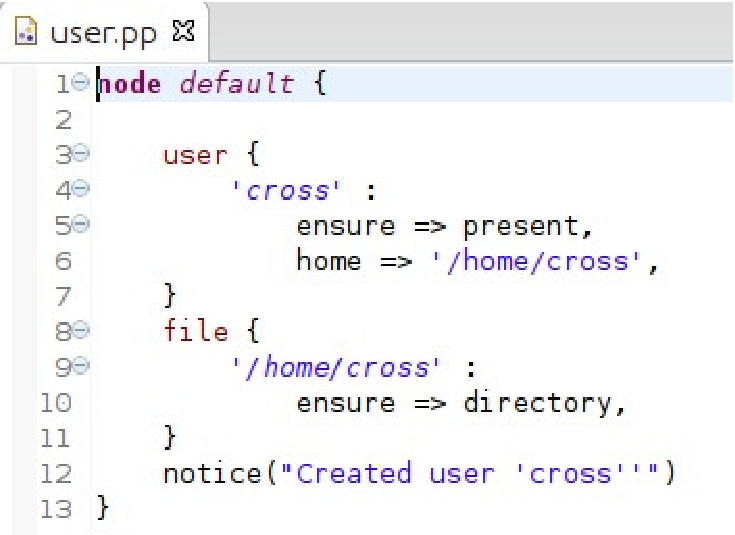
\includegraphics[width=0.5\textwidth]{images/user.pdf}
  \end{center}
  \caption{User mit Puppet anlegen}
\end{wrapfigure}

\bibliographystyle{apalike2}
\bibliography{document}

\end{document}
